\documentclass[dvipdfmx]{article}
\usepackage[dvipdfmx]{graphicx}
\usepackage{amsmath, amssymb}
\usepackage{mathtools}
\usepackage{here}
\begin{document}
\title{Weekly Report}
\author{Riku Gondow}
\maketitle
\section{Progress}
\begin{itemize}
    \item Revise bachelor thesis, especially examine the noise contained in the signal.
    \item After the BPF was applied, the wavelet reconstruction was carried out.
\end{itemize}

\subsection{Noise contained in the signal}
To see if the frequencies attributed to the heartbeat were extracted, I used the Welch method to examine the frequency response.

\begin{figure}[htbp]
    \begin{minipage}[c]{0.5\hsize}
      \centering
      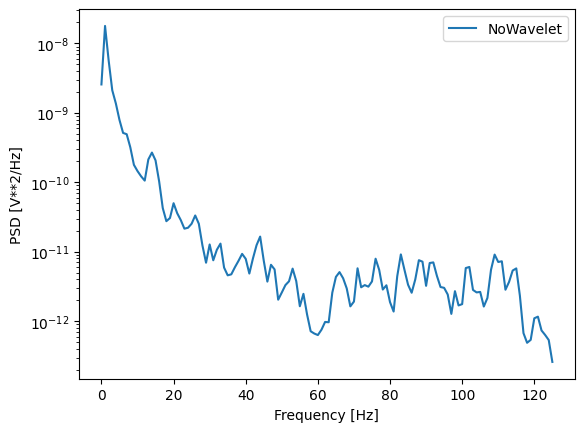
\includegraphics[width=\linewidth]{./img/welch_nowavelet.png}
      \caption{Frequency-power spectral characteristics before wavelet reconstruction}
    %   \label{fig:statue}
    \end{minipage}
    \begin{minipage}[c]{0.5\hsize}
      \centering
      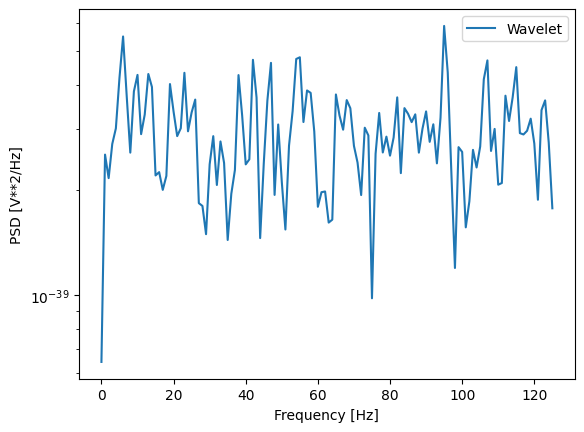
\includegraphics[width=\linewidth]{./img/welch_wavelet.png}
      \caption{Frequency-power spectral characteristics after wavelet reconstruction}
    %   \label{fig:spaceship}
    \end{minipage}
\end{figure}
After wavelet reconstruction, the overall power was lower, and the power in the 0.6-2 Hz frequency band, which is the frequency of a heartbeat, and the power in the higher frequency band were similar.

\subsection{Try BPF + Wavelet Reconstruction}
Since the frequency response after wavelet reconstruction did not extract well the 0.6-2 Hz frequency band corresponding to the heartbeat frequency band, the BPF was applied before wavelet reconstruction.

\begin{figure}[H]
\begin{center}
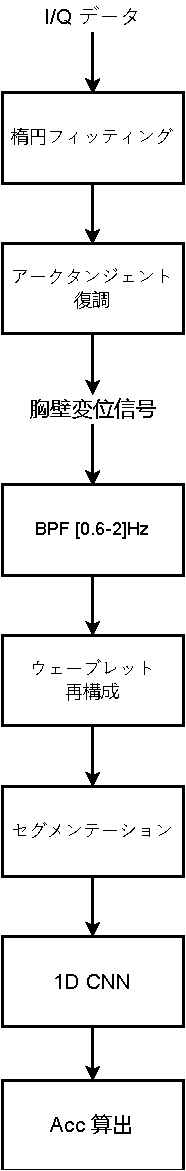
\includegraphics[width=0.2\linewidth]{./img/proposed_method.drawio_addBPF.pdf}
\end{center}
\caption{The algorithm of proposed method}
\end{figure}

\begin{figure}[htbp]
    \begin{minipage}[c]{0.5\hsize}
      \centering
      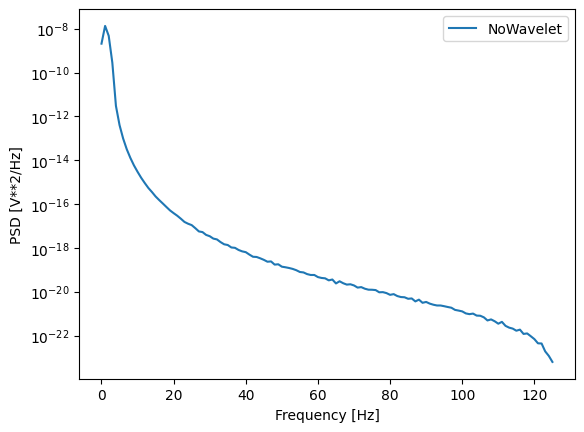
\includegraphics[width=\linewidth]{./img/BPF_welch.png}
      \caption{Frequency response of chest wall displacement signal with BPF applied}
    %   \label{fig:statue}
    \end{minipage}
    \begin{minipage}[c]{0.5\hsize}
      \centering
      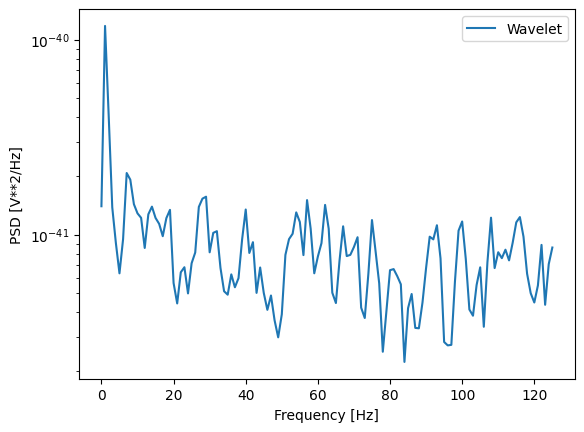
\includegraphics[width=\linewidth]{./img/BPF_wavelet_welch.png}
      \caption{Frequency response of chest wall displacement signal using BPF and wavelet reconstruction}
    %   \label{fig:spaceship}
    \end{minipage}
\end{figure}

On the Keio Hospital dataset, which consists of 12 subjects, we achieved 93.82\% accuracy under the close-set condition(Cross-validation is not performed). The confusion matrix is shown below.

\begin{figure}[H]
\begin{center}
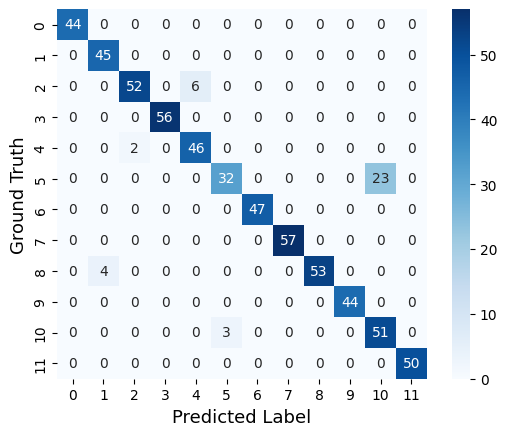
\includegraphics[width=0.8\linewidth]{./img/conf_bpf_wavelet.png}
\end{center}
\caption{Confusion Matrix when applying BPF + Wavelet Reconstruction}
\end{figure}

\section{Next Plan}
\begin{itemize}
    \item Pass BPF after applying Wavelet Reconstruction
\end{itemize}
\end{document}
